\documentclass[aspectratio=169,12pt]{beamer}
\usepackage[utf8]{inputenc}
\usepackage[spanish, es-nodecimaldot]{babel}
%\usepackage{icomma} % Use dot as decimal separator
\usepackage{booktabs} % For better-looking tables
\usepackage{wrapfig}
%\usepackage{siunitx}

\usepackage{multicol}
\usepackage{mathtools}

\usepackage[normalem]{ulem}

\pagestyle{empty}

\usepackage{pgf,tikz}
\usepackage{pgfplots}
\usetikzlibrary{matrix}
\usetikzlibrary{arrows}

%\usepackage{wrapfig}
\mode<presentation>
\usefonttheme{professionalfonts}
\usetheme{Darmstadt}
\usecolortheme{orchid}
\useoutertheme{default}
\setbeamertemplate{headline}{}

\renewcommand{\baselinestretch}{1.1}

%gets rid of bottom navigation bars
\setbeamertemplate{footline}[page number]

%gets rid of navigation symbols
\setbeamertemplate{navigation symbols}{}

%\frameframe{none} % No default frame

%\setlength{\framewidth}{8.7in} \setlength{\frameheight}{7.2in}

\parindent 0pt
\setlength{\parskip} {1ex plus 0.5ex minus 0.2ex}


%\usepackage[bbgreekl]{mathbbol}
\usepackage{amsfonts}

%\DeclareSymbolFontAlphabet{\mathbb}{AMSb}
%\DeclareSymbolFontAlphabet{\mathbbl}{bbold}

\newcommand{\Sym}{{\mathcal S}}
\DeclareMathOperator{\Aut}{Aut}
\DeclareMathOperator{\Tr}{Tr}
\DeclareMathOperator{\trace}{Trace}
\DeclareMathOperator{\range}{range}
\DeclareMathOperator{\rank}{rank}

\usepackage{breqn}
\usepackage{multicol}
\usepackage{colortbl}
\usepackage{lmodern}
\usepackage{tabularx}
\usepackage{multirow}
\usepackage{amssymb}
\usepackage{amsmath}
\usepackage{stmaryrd}
\usepackage{color}
\usepackage{graphicx}
\graphicspath{ {img/} }
\usepackage{hyperref}

\input{epsf}
\title{Introducción}
\author{}

\DeclareMathOperator{\Hom}{Hom}
\DeclareMathOperator{\sing}{sing}

\DeclareMathOperator{\chara}{char}
\DeclareMathOperator{\Jacob}{Jacob}
\DeclareMathOperator{\Sing}{Sing}
\newcommand{\fracNoLine}[2]{\genfrac{}{}{}{0pt}{#1}{#2}}

%\beamerdefaultoverlayspecification{<+->}

\usepackage{listings,xcolor,bm}


\definecolor{mygreen}{rgb}{0,0.6,0}
\definecolor{mygray}{rgb}{0.5,0.5,0.5}
\definecolor{mymauve}{rgb}{0.58,0,0.82}
\lstset{
  backgroundcolor=\color{white},   % choose the background color; you must add
  basicstyle=\small\ttfamily,      % the size of the fonts that are used for the code
  breakatwhitespace=false,         % sets if automatic breaks should only happen at whitespace
  breaklines=true,                 % sets automatic line breaking
  captionpos=b,                    % sets the caption-position to bottom
  commentstyle=\color{mygreen},    % comment style
  deletekeywords={...},            % if you want to delete keywords from the given language
  escapeinside={\%*}{*)},          % if you want to add LaTeX within your code
  extendedchars=true,              % lets you use non-ASCII characters; for 8-bits encodings only, does not work with UTF-8
  firstnumber=1,                % start line enumeration with line 1000
  frame=single,	                   % adds a frame around the code
  keepspaces=true,                 % keeps spaces in text, useful for keeping indentation of code (possibly needs columns=flexible)
  keywordstyle=\color{blue},       % keyword style
  language=Python,                 % the language of the code
  morekeywords={*,...},            % if you want to add more keywords to the set
  numbers=left,                    % where to put the line-numbers; possible values are (none, left, right)
  numbersep=5pt,                   % how far the line-numbers are from the code
  numberstyle=\tiny\color{mygray}, % the style that is used for the line-numbers
  rulecolor=\color{black},         % if not set, the frame-color may be changed on line-breaks within not-black text (e.g. comments (green here))
  showspaces=false,                % show spaces everywhere adding particular underscores; it overrides 'showstringspaces'
  showstringspaces=false,          % underline spaces within strings only
  showtabs=false,                  % show tabs within strings adding particular underscores
  stepnumber=5,                    % the step between two line-numbers. If it's 1, each line will be numbered
  stringstyle=\color{mymauve},     % string literal style
  tabsize=4,	                   % sets default tabsize to 2 spaces
  title=\lstname                   % show the filename of files included with \lstinputlisting; also try caption instead of title
}

\begin{document}

\newtheorem{prop}{Proposici\'on}
\newtheorem{algo}[prop]{Algorithm}
\newtheorem{teor}[prop]{Theorem}
\newtheorem{lema}[prop]{Lemma}
\newtheorem{coro}[prop]{Corollary}
\newtheorem{defi}[prop]{Definition}

\newcommand{\ideal}[1]{{\left\langle{#1}\right\rangle}}
\newcommand{\demo}{\textbf {Demostraci\'on. }}
\newcommand{\obse}{\textbf {Observaci\'on. }}
\newcommand{\Input}{\textbf {Input: }}
\newcommand{\Output}{\textbf {Output: }}
\newcommand{\Examp}{\textbf {Ejemplo }}
\newcommand{\Examps}{\textbf {Ejemplos }}

\newcommand{\kk}{{\mathbbl k}}
\newcommand{\V}{{\mathbf V}}
\newcommand{\I}{{\mathbf I}}
\newcommand{\PP}{{\tilde P}}
\newcommand{\QQ}{{\tilde Q}}

\newcommand{\F}{{\mathbb F}}
\newcommand{\Q}{{\mathbb Q}}
\newcommand{\N}{{\mathbb N}}
\newcommand{\R}{{\mathbb R}}
\newcommand{\Z}{{\mathbb Z}}
\newcommand{\CC}{{\mathbb C}}
\newcommand{\eLL}{{\mathcal L}}



\newcommand{\MinAss}{\textrm {MinAss}}
\newcommand{\Ass}{\textrm {Ass}}
\newcommand{\mcm}{\textrm {mcm}}
\newcommand{\mcd}{\textrm {mcd}}
%\newcommand{\mod}{\textrm { mod }}
\newcommand{\lt}{\textrm {lt}}
\newcommand{\Lt}{\textrm {Lt}}
\newcommand{\lp}{\textrm {lp}}
\newcommand{\lc}{\textrm {lc}}
\newcommand{\lm}{\textrm {lm}}
\newcommand{\barra}{\ /\ }
\newcommand{\multideg}{\textrm {multideg}}

\newcommand{\sep}{\textrm {sep}}
\newcommand{\Syz}{\textrm {Syz}}
\newcommand{\n}{\~n}
\newcommand{\cG}{\textrm {cG}}
\newcommand{\dG}{\textrm {dG}}
\newcommand{\nG}{\textrm {nG}}
\newcommand{\CE}{\textrm {CE}}
\newcommand{\CG}{\textrm {CG}}
\newcommand{\CF}{\textrm {CF}}
\newcommand{\DG}{\textrm {DG}}
\renewcommand{\NG}{\textrm {NG}}

\newcommand{\p}{{\boldsymbol{p}}}
\newcommand{\q}{{\boldsymbol{q}}}

\newcommand{\X}{{\boldsymbol{X}}}
\newcommand{\x}{{\boldsymbol{x}}}
\renewcommand{\u}{{\boldsymbol{u}}}
\renewcommand{\t}{{\boldsymbol{t}}}
\renewcommand{\a}{{\boldsymbol{a}}}
\renewcommand{\b}{{\boldsymbol{b}}}
\renewcommand{\c}{{\boldsymbol{c}}}

%Titulos en espa�ol
%\renewcommand{\chaptername}{Cap\'{\i}tulo}
%\renewcommand{\bibname}{Bibliograf\'{\i}a}

\newcommand{\kring}{\kk[\x]}
\newcommand{\kRing}{\kk[X]}
\newcommand{\qring}{\Q[\x]}

%\renewcommand\itemindent{-10pt}
%\renewcommand{\theenumi}{\arabic{enumi}}
%\renewcommand{\labelenumi}{\Alph{enumi}}

\definecolor{issac}{rgb}{1.00,0.00,0.00}
%------------------------------------------------------------------

\begin{frame}

 \begin{center}

\Large\textbf{Laboratorio de Datos} \\
\large\textbf{Entrenamiento y testeo}
%\vspace{0.5cm}

% \textit{Santiago Laplagne} \\
%slaplagn@dm.uba.ar \\


%\vspace{0.5cm}
%{\small Trabajo en progreso en conjunto con \emph{Jose Capco} (Universit\"at Innsbruck) y \emph{Claus Scheiderer} %(Universit\"at Konstanz).} \\

\vspace{1cm}
Primer Cuatrimestre 2024 \\ Turnos tarde y noche

\vspace{1cm}


 {\small Facultad de Ciencias Exactas y Naturales, UBA}
 \end{center}


\end{frame}

%------------------------------------------------------------------

\begin{frame}
\frametitle{Introducción: sistemas de ecuaciones lineales}

Sabemos que un fonde de inversión invirtió en acciones de YPF, Santander y Nvidia (y solo en estas acciones) pero no sabemos cuántas acciones compró de cada una. ¿Cómo podemos averiguarlo? 

\pause

Suponemos que tenemos disponible:
\begin{itemize}
\item La valorización del fondo al final de cada día.
\item El valor la acción de cada empresa al cierre de cada día. 
\end{itemize}

\end{frame}

%------------------------------------------------------------------

\begin{frame}
\frametitle{Sistemas de ecuaciones lineales}

Ponemos toda la información en la siguiente tabla.

\begin{table}[h]
    \centering
    \begin{tabular}{|c|c|c|c|}
        \hline
        Total & YPF & Santander & Nvidia \\
        \hline
        170262.00 & 20935 & 20100 & 37100.0 \\
        169929.50 & 21030 & 20500 & 36255.0 \\
        171064.00 & 20770 & 21700 & 36000.0 \\
        169637.35 & 20950 & 21000 & 35645.5 \\
        164625.45 & 20750 & 20316 & 33878.5 \\
        \hline
    \end{tabular}
    \caption{Valores diarios de acciones}
    \label{tab:my_table}
\end{table}

\end{frame}

%------------------------------------------------------------------

\begin{frame}
\frametitle{Planteamos el sistema lineal}

Llamamos $c_1$, $c_2$ y $c_3$ a la cantidad de acciones de cada tipo.
Para calcular los valores, tenemos que resolver el siguiente sistema de ecuaciones:

\begin{align*}
& \quad YPF \quad \ Santander \quad Nvidia \\
& \quad \quad \downarrow \quad  \quad  \quad  \quad \downarrow  \quad  \quad \quad \quad \downarrow  \\
\text{D\'ia 1} \rightarrow \quad 170262.00	&= 20935	c_1 + 20100 c_2 + 37100.0 c_3 \\
\text{D\'ia 2} \rightarrow \quad 169929.50	&= 21030	c_1 + 20500 c_2 + 36255.0 c_3 \\
\text{D\'ia 3} \rightarrow \quad 171064.00	&= 20770	c_1 + 21700 c_2 + 36000.0 c_3 \\
\text{D\'ia 4} \rightarrow \quad 169637.35	&= 20950	c_1 + 21000 c_2 + 35645.5 c_3 \\
\text{D\'ia 5} \rightarrow \quad 164625.45	&= 20750	c_1 + 20316 c_2 + 33878.5 c_3 \\
\end{align*}

\end{frame}

%------------------------------------------------------------------

\begin{frame}
\frametitle{Resolvemos el sistema}

Como tenemos 3 incógnitas, nos alcanza con 3 ecuaciones:
\begin{align*}
170262.00	&= 20935	c_1 + 20100 c_2 + 37100.0 c_3 \\
169929.50	&= 21030	c_1 + 20500 c_2 + 36255.0 c_3 \\
171064.00	&= 20770	c_1 + 21700 c_2 + 36000.0 c_3
\end{align*}

Para resolver el sistema, construimos la matriz ampliada

$$ 
\left(\begin{array}{ccc|c}
20935.0	& 20100.0 & 37100.0 & 170262.00	 \\
21030.0	& 20500.0 & 36255.0 & 169929.50	 \\
20770.0	& 21700.0 & 36000.0 & 171064.00	
\end{array}\right) 
$$

\vspace{0.5cm}

¿Qué hay en las primeras 3 columnas de la matriz? ¿Qué hay en la última columna?

\end{frame}

%------------------------------------------------------------------

\begin{frame}
\frametitle{Solución del sistema}

Triangulando la matriz y despejando, obtenemos los valores
$$
c_1 = 3.2, \quad \quad c_2 =  2.0, \quad \quad c_3 = 1.7.
$$

Estas son las cantidades de cada acción que tiene el fondo de inversión.

\end{frame}

%------------------------------------------------------------------

\begin{frame}
\frametitle{Notación matricial}

Podemos escribir el sistema de ecuaciones
en forma compacta usando notación matricial:
$$
\begin{pmatrix}
20935.0	& 20100.0 & 37100.0 \\
21030.0	& 20500.0 & 36255.0 \\
20770.0	& 21700.0 & 36000.0
\end{pmatrix}
\begin{pmatrix}
c_1 \\
c_2 \\
c_3
\end{pmatrix} = 
\begin{pmatrix}
170262.00 \\
169929.50 \\
171064.00
\end{pmatrix}
$$

Obtenemos un sistema de la forma
$$
X c = y
$$

¿Qué hay en las columnas de $X$? ¿Que hay en la matriz $y$?



\end{frame}

%------------------------------------------------------------------

\begin{frame}
\frametitle{Verificación del ``modelo''}

En base a los resultados que obtuvimos, ¿podemos confirmar que las acciones del fondo son las 3 acciones que usamos?

Si no estamos seguros si eran acciones de Santander o Galicia, ¿cómo podríamos asegurarnos?

Cambiamos los valores de Santander por los valores de Galicia:
\begin{align*}
170262.00	&= 20935	c_1 + {\bf 20100} c_2 + 37100.0 c_3 \\
169929.50	&= 21030	c_1 + {\bf 19400} c_2 + 36255.0 c_3 \\
171064.00	&= 20770	c_1 + {\bf 21900} c_2 + 36000.0 c_3
\end{align*}


\end{frame}


%------------------------------------------------------------------

\begin{frame}
\frametitle{Sobreajuste}

Resolvemos el sistema y obtenemos estos valores:
$$c_1 = 6.69507872, \quad \quad c_2 = 1.16828332, \quad \quad c_3 = 0.17838362$$

Los números no se ven menos redondos, pero eso no alcanza para decidir cuál es el modelo correcto.

Un sistema de 3 ecuaciones y 3 incógnitas en general \textbf{siempre} tiene solución.

\textbf{Sobreajuste (overfitting).} Cuando tenemos igual cantidad de parámetros que observaciones, el sistema (casi) siempre va a tener solución pero no nos da ninguna información sobre si el modelo es correcto, no podemos usarlo para estimar otros valores.

\end{frame}


%------------------------------------------------------------------

\begin{frame}
\frametitle{Selección de modelos}

¿Qué estrategias se les ocurren para ver cuál modelo es mejor? \pause

\begin{enumerate}
\item Verificar la fórmula en otros días. \pause
\item Utilizar más días al plantear el sistema de ecuaciones.
\end{enumerate}

\pause

Las dos estretegias son ideas centrales en la construcción de modelos:
\begin{enumerate}
\item Probar el modelo en datos distintos a los que usamos para construir el modelo.
\item Utilizar la mayor cantidad posible de datos para construir el modelo.
\end{enumerate}

\end{frame}


%------------------------------------------------------------------

\begin{frame}
\frametitle{1. Conjuntos de entrenamiento y testeo}

Separamos nuestro conjunto de datos en dos subconjuntos:
\begin{itemize}
\item \textbf{Conjunto de entrenamiento.} Lo utilizamos para construir el modelo. En un modelo lineal, lo usamos para calcular los coeficientes ($c_1, c_2, c_3$).
\item \textbf{Conjunto de testeo.} Lo utilizamos para verificar si el modelo construido ajusta bien a los datos en este conjunto.
\end{itemize}

\end{frame}


%------------------------------------------------------------------

\begin{frame}
\frametitle{2. Más ecuaciones que variables - Ejemplo de juguete}

Si consideramos el sistema original, tenemos 5 ecuaciones y 3 variables.

\begin{align*}
& \quad YPF \quad \ Santander \quad Nvidia \\
& \quad \quad \downarrow \quad  \quad  \quad  \quad \downarrow  \quad  \quad \quad \quad \downarrow  \\
\text{D\'ia 1} \rightarrow \quad 170262.00	&= 20935	c_1 + 20100 c_2 + 37100.0 c_3 \\
\text{D\'ia 2} \rightarrow \quad 169929.50	&= 21030	c_1 + 20500 c_2 + 36255.0 c_3 \\
\text{D\'ia 3} \rightarrow \quad 171064.00	&= 20770	c_1 + 21700 c_2 + 36000.0 c_3 \\
\text{D\'ia 4} \rightarrow \quad 169637.35	&= 20950	c_1 + 21000 c_2 + 35645.5 c_3 \\
\text{D\'ia 5} \rightarrow \quad 164625.45	&= 20750	c_1 + 20316 c_2 + 33878.5 c_3
\end{align*}

En este ejemplo (de juguete) si utilizamos los datos de Santander, el sistema tiene solución.
Si usamos los datos de Galicia el sistema no tiene solución.

\end{frame}


%------------------------------------------------------------------

\begin{frame}
\frametitle{2. Más ecuaciones que variables - La vida real}

Cuando consideramos un sistema con más ecuaciones que variables, en general \textbf{NO} tiene solución.

Aunque teóricamente exista solución, en la práctica siempre aparecen errores numéricos y no podemos determinar si un sistema tiene solución (numéricamente es MUY difícil saber si un número es igual a 0 o no).

Solución: en vez de buscar una solución exacta del sistema de ecuaciones
$$ X c = y,$$
buscamos un vector $c$ que minimice el error, es decir, que haga pequeñas las coordenadas del vector de errores
$$ X c - y.$$

\end{frame}


%------------------------------------------------------------------

\begin{frame}
\frametitle{El milagro de los mínimos cuadrados}

Llegamos así al método de mínimos cuadrados. El vector $c$ que  minimiza la suma de los errores al cuadrado del sistema
$$ X c = y,$$
es solución del sistema lineal de ecuaciones
$$ X^T X c = X^T y.$$

Es un sistema cuadrado y en general tiene solución única. 

El problema DIFICIL de minimizar los errores se transforma en el problema FÁCIL de resolver un sistema lineal de ecuaciones. \textbf{Este es el milagro de los mínimos cuadrados.}

\end{frame}

%------------------------------------------------------------------

\begin{frame}
\frametitle{Resumen}

Tenemos dos modelos posibles y queremos elegir el más apropiado:
\begin{align*}
A) total &= c_1 \cdot YPF + c_2 \cdot Santander + c_3 \cdot Nvidia \\
B) total &= c_1 \cdot YPF + c_2 \cdot Galicia + c_3 \cdot Nvidia
\end{align*}

Seguimos los siguientes pasos:
\begin{enumerate}
\item Buscamos datos de la mayor cantidad posible de días.
\item Separamos el conjunto en dos: conjunto de entrenamiento ($80\%$ de los días) y conjunto de testeo ($20\%$ restante)
\item Calculamos $c_1, c_2, c_3$ para cada uno de los dos modelos utilizando mínimos cuadrados en el conjunto de entrenamiento.
\item Calculamos el error cuadrático medio de lás fórmulas resultantes aplicadas al conjunto de testeo.
\end{enumerate}

\end{frame}

%------------------------------------------------------------------

\begin{frame}
\frametitle{Modelo lineal multivariado}

El caso recién visto fue un ejemplo de juguete, donde existe una relación lineal entre las variables que tenemos que estimar.

En las aplicaciones reales, esa formula puede no existir (por ejemplo, si queremos estimar los gastos en tarjeta de crédito de una persona en función del sueldo y la cantidad de hijos), pero el modelo lineal puede darnos una buena estimación.

En el modelo lineal suponemos que existe una relación del tipo
$$ X c = y.$$

Como esa relación en general no existe, buscamos un vector $c$ que haga que $X c$ se parezca lo más posible a $y$.

\end{frame}

%------------------------------------------------------------------

\begin{frame}
\frametitle{Ejercicio: modelos lineales}

Dadas una variable a predecir $y$ y variables explicativas $x_1, x_2, \dots$, ¿cuáles de los siguientes modelos son lineales? ¿Cuál es la matriz $X$ en cada caso?

\begin{enumerate}
\item $y = c_0 + c_1 x_1 + c_2 x_2$
\item $y = c_0 + c_1 x_1 + c_2 x_1^2$
\item $y = c_0 + c_1 x_1 + x_1^{c_2}$
\item $y = c_0 + c_1 x_1 + c_2 x_2 + c_3 x_1 x_2$
\item $y = c_0 + c_1 \sin(x_1) + c_2 \sin(x_2)$
\item $y = c_0 + c_1 \sin(c_2 + x_1)$
\item $y = c_0 + c_1 e^{x_1}$
\item $y = c_0 \cdot c_1 ^{x_1}$
\end{enumerate}

\end{frame}
 %------------------------------------------------------------------

\begin{frame}
\frametitle{Ejemplo real: cálculo de calorías}

Vamos a repetir estos pasos en un caso real: calculas las calorías de un alimento en función de sus componentes, utilizando las herramientas de Python para la construcción de modelos.
\begin{enumerate}
\item Construimos las matrices $X$ e $y$ utilizando \lstinline{Formulaic}.
\item Separamos las matrices en entrenamiento y testeo utilizando \lstinline{train_test_split}
\item Ajustamos el modelo utilizando \lstinline{linear_model.fit()}.
\item Calculamos el error en los datos de testeo utilizando \lstinline{linear_model.predict()}.
\end{enumerate}

\end{frame}


%------------------------------------------------------------------

\begin{frame}
\frametitle{Box plot}

Un gráfico \textbf{box plot} usa cajas y líneas para mostrar información de la distribución de uno o más grupos de datos numéricos.

\begin{center}
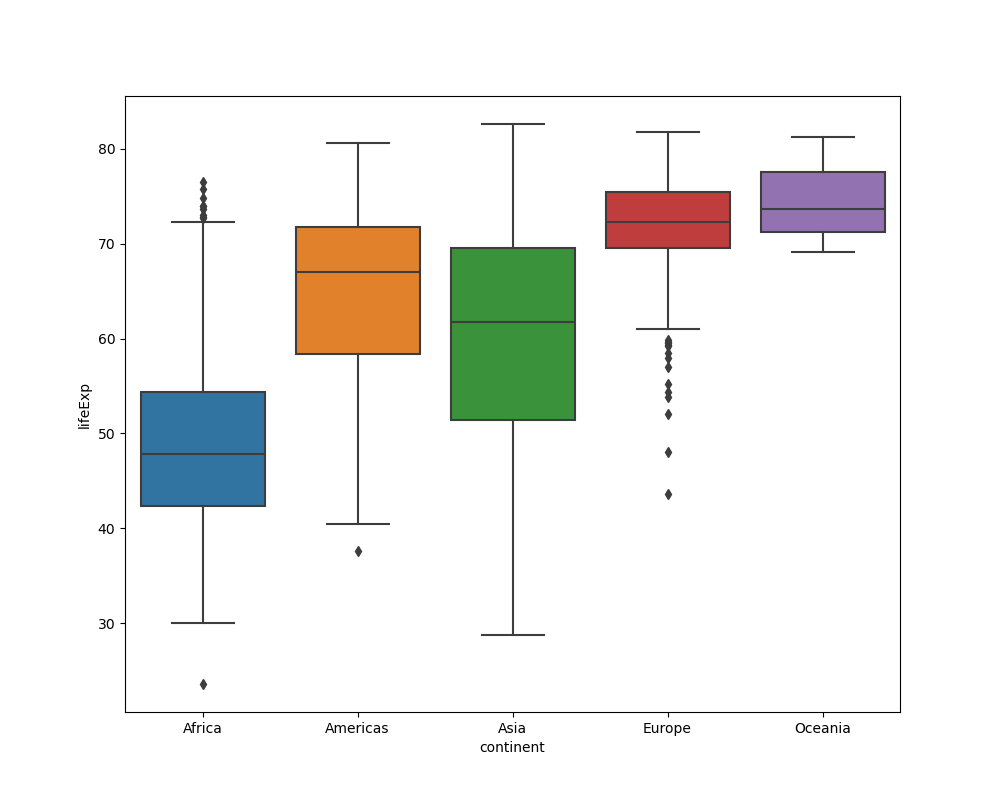
\includegraphics[scale=.3]{practica3-img-gapminder-boxplot.png}
\end{center}

\end{frame}

%------------------------------------------------------------------

\begin{frame}
\frametitle{Elementos de un Box plot: cuartiles}

Dada una variable numérica, ordenamos los valores y los partimos en 4 grupos de igual tamaño.

\begin{itemize}
\item Primer cuartil (Q1): es un valor mayor que el $25\%$ de los datos y menor que el otro $75\%$.
\item Segundo cuartil (Q2): es un valor mayor que el $50\%$ de los datos y menor que el otro $50\%$ (corresponde a la mediana).
\item Tercer cuartil (Q3): es un valor mayor que el $75\%$ de los datos y menor que el otro $25\%$.
\end{itemize}

\begin{center}
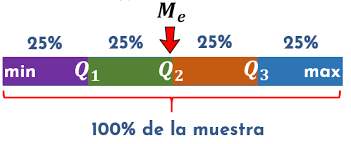
\includegraphics[scale=.5]{clase4-cuartiles-esquema.png}
\end{center}



%En un box plot, dibujamos una caja, con límites en Q1 y Q3 y una línea central marcando el valor de Q2.

\end{frame}

%------------------------------------------------------------------

\begin{frame}
\frametitle{Cuartiles: ejemplo}

Ordenamos los datos de menor a mayor y tomamos valores que dividen a los datos en 4 partes iguales.

\begin{center}
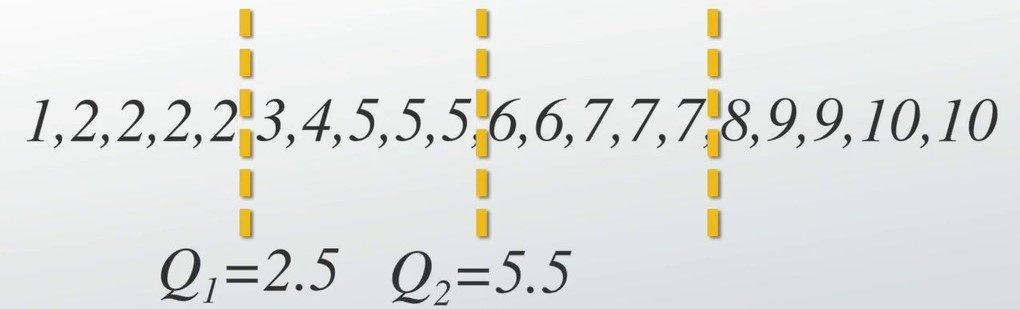
\includegraphics[scale=.3]{clase4-cuartiles-Q1yQ2.jpg}
\end{center}
%En un box plot, dibujamos una caja, con límites en Q1 y Q3 y una línea central marcando el valor de Q2.

\end{frame}

%------------------------------------------------------------------

\begin{frame}
\frametitle{Cálculo de cuartiles en Wikipedia...}

\begin{center}
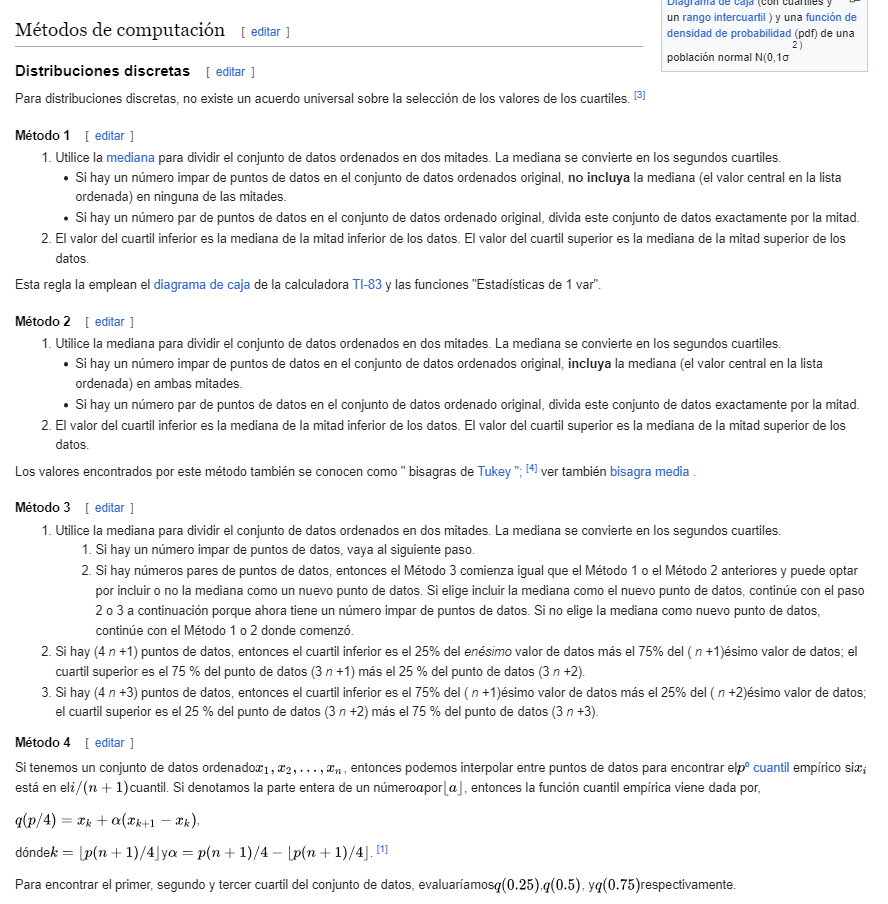
\includegraphics[scale=.3]{clase4-cuartiles.png}
\end{center}

\end{frame}

%------------------------------------------------------------------

%\begin{frame}
%\frametitle{Box plot}
%
%Un gráfico \textbf{box plot} usa cajas y líneas para mostrar información de la distribución de uno o más grupos de datos numéricos.
%
%\begin{center}
%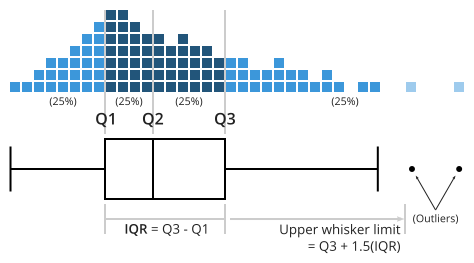
\includegraphics[scale=.5]{clase4-box-plot-construction.png}
%\end{center}
%
%\end{frame}

%------------------------------------------------------------------

\begin{frame}
\frametitle{Elementos de un Box plot}

Dada una variable numérica, ordenamos los valores y los partimos en 4 grupos de igual tamaño.

En un box plot, dibujamos una caja, con límites en Q1 y Q3 y una línea central marcando el valor de Q2.

\begin{center}
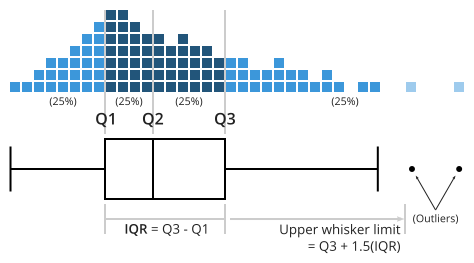
\includegraphics[scale=.45]{clase4-box-plot-construction.png}
\end{center}

\end{frame}

%------------------------------------------------------------------

\begin{frame}
\frametitle{Elementos de un Box plot}

La distancia entre Q3 y Q1 se conoce como \emph{rango intercuartil} (IQR) y se utilizan para trazar los "bigotes".

Cada bigote se extiende hasta el valor más lejano de los datos a una distancia menor a $1.5$ veces el valor IQR.

Cualquier valor de los datos más allá de esa distancia se considera un dato atípico (outlier) y se marca con un punto.

\begin{center}
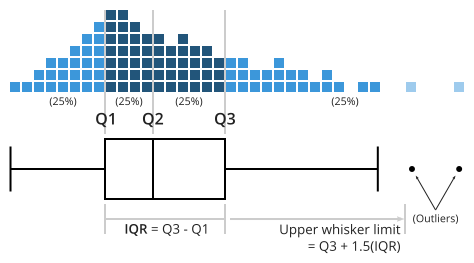
\includegraphics[scale=.35]{clase4-box-plot-construction.png}
\end{center}

\end{frame}



\end{document}

